\sub{Speichern der generierten Daten}
Um NutzerInnenspezifische Daten offline verfügbar zu machen können sie im Browser gespeichert werden. Einige Methoden hierfür werden im Folgenden erläutert.
%
\subsub{Web Storage}
Das Web Storage \gls{API} ist ein Web-Standard mit dessen Hilfe Daten als Schlüssel / Wert Paare im Browser gespeichert werden können. Es wird, wie Abbildung \ref{fig:webStorage} zeigt, von allen, bis auf den Opera Mini,  Browsern unterstützt. Opera Mini speichert grundsätzlich keine Daten, weswegen dieser Browser auch in den nachfolgenden Bildern mit Rot markiert ist.
Web Storage umfasst zwei Mechanismen. Den Session Storage und den Local Storage.\\
Der Session Storage existiert nur so lange der Browser geöffnet ist.
Das heißt alle Daten die im Session Storage gespeichert werden, existieren nicht mehr sobald der Browser geschlossen wird. Daten die im Local Storage gespeichert sind, existieren dort solange bis der Browser Cache geleert wird~\cite{webstorage}.
\begin{figure}[H]
	\centering
	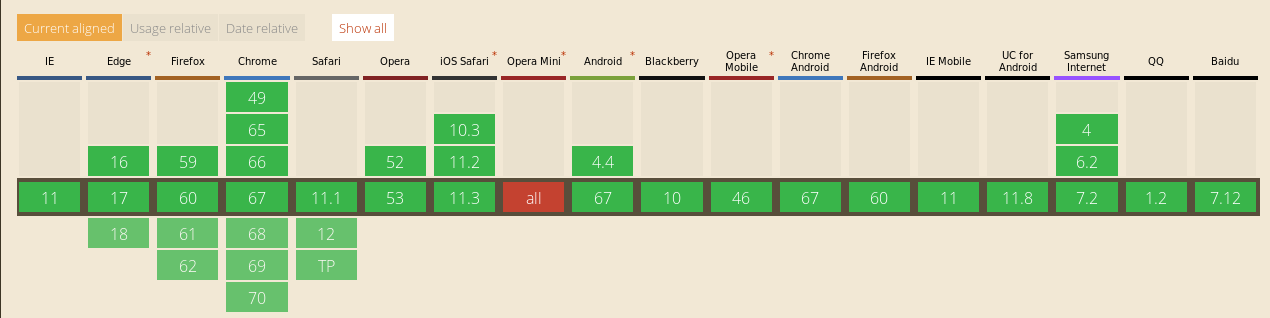
\includegraphics[width=\textwidth]{webStorage}
	\grayRule
	\caption[Browserkompatibilität für Web Storage]{Browserkompatibilität für Web Storage, Quelle: ~\cite{caniuse-ws}}
	\label{fig:webStorage}
\end{figure}
Der von den Browsern freigegebene Cache-Space für Web Storage variiert, ist aber meist auf 10 MB begrenzt. Der größte Nachteil ist wohl, dass Web Storage synchron arbeitet und so andere Operationen, wie zum Beispiel das Rendern der Seite, blockieren kann ~\cite{webstorage-con}.
%
%
\subsub{Web SQL}
Eine andere der lokalen Speicherung im Browser ist die Web SQL Datenbank.
Sie hat ein asynchrones \gls{API} und unterstützt die grundlegenden SQL Abfragen. Web SQL sollte in den W3C Standards aufgenommen werden. Aus Mangel unabhängigen Implementierungen wie eine andere \gls{DB} als SQLite im Backend wurde es abgelehnt~\cite{websql}.\\
Das Web SQL \gls{API} wird nur von den Webkit--Browsern unterstützt. Also nicht von Firefox, dem Internet Explorer oder dessen neueren Variante Edge~\cite{caniuse-websql}.
%
%
\subsub{IndexedDB}
IndexedDB ist eine weitere Variante der clientseitigen Datenspeicherung. Die auf Java"-Script basierende, objektorientierte Datenbank erlaubt neben dem Speichern von größeren Datenmengen in Form von Objekten auch das Speichern von Dateien. Durch die Verwendung von Indizes lassen sich Objekte schnell speichern und finden. Das asynchrone \gls{API} erlauben Datenbankabfragen die keinen anderen Prozess blockieren~\cite{idb}.
\begin{figure}[H]
	\centering
	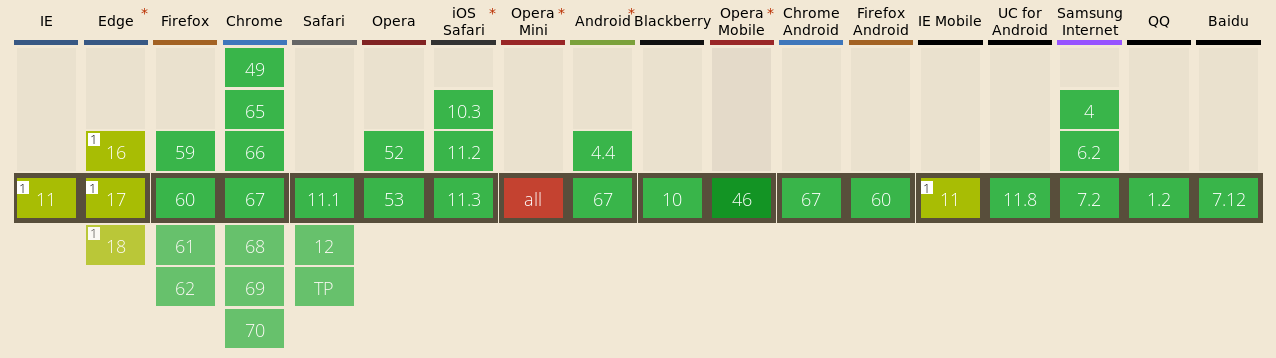
\includegraphics[width=\textwidth]{indexedDB}
	\grayRule
	\caption[Browserkompatibilität für IndexedDB]{Browserkompatibilität für IndexedDB, Quelle: ~\cite{caniuse-idb}}
	\label{fig:indexedDB}
\end{figure}
Wie in Abbildung \ref{fig:indexedDB} zu sehen ist, wird IndexedDB von allen gängigen Browsern unterstützt. 
%
\subsub{IndexedDB 2.0}
Im Januar 2018 wurde die zweite Version des IndexedDB \glspl{API} zur W3C Spezifikation hinzugefügt. Es erweitert die erste Verion um Funktionalität und verbessert die Performance~\cite{idb2}.
Die Aktualität dieser Spezifikation spiegelt sich in der Browserunterstützung wider. Die Abbilung \ref{fig:indexedDB2} zeigt, dass die zweite Version nur von den beliebten \highlight{(haha)} Desktopbrowsern und einigen mobilen Browsern unterstützt wird. 
\begin{figure}[H]
	\centering
	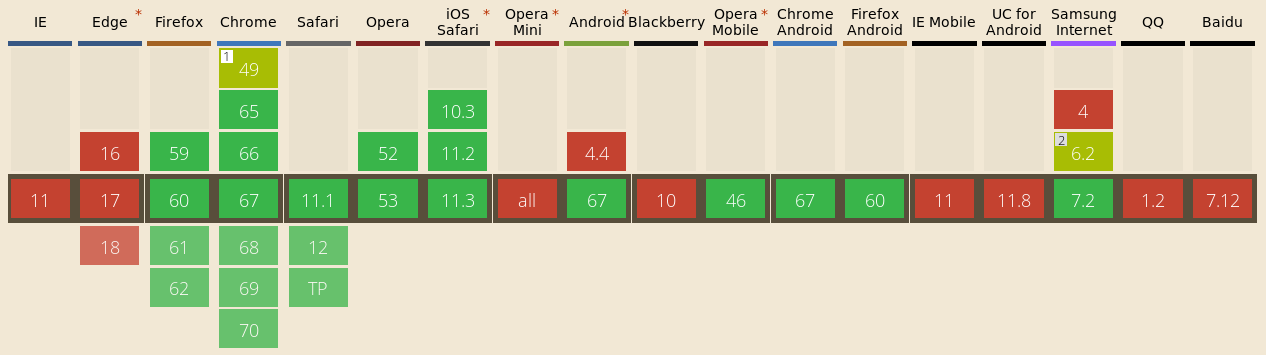
\includegraphics[width=\textwidth]{indexedDB2}
	\grayRule
	\caption[Browserkompatibilität für IndexedDB 2.0]{Browserkompatibilität für IndexedDB 2.0, Quelle: ~\cite{caniuse-idb}}
	\label{fig:indexedDB2}
\end{figure}
IndexedDB wird stetig weiterentwickelt und es gibt bereits einen Spezifikationsentwurf für die dritte Version~\cite{idb3}. 